\section{Learning and testing five-listing recommendations}\label{sec:learned}
We train on 1,920 summer markets (122,880 renter outcomes) and select epochs on a separate 384. Each label is a partner or the outside option in full-exposure DA. Each feasible edge has five features: rent relative to the budget, spare bedrooms, distance, listing quality and the capped income-to-annual-rent ratio. The network sees eligibility and these features. Neither actual simulated priority draws nor renter or listing identifiers enter its predictions. The score for a listing can depend on the other renters competing for it. Two rounds of message passing average the feasible edge representations for each renter and each listing; separate heads score the edge and the outside option. We minimize cross-entropy over feasible listings and the outside option and average the predictions from three validation-selected fits. The basic pointwise comparison removes competition messages. Appendix~\ref{app:ai} describes the architecture, capacity control and precision checks.

We froze all policies and tested on 48 new summer blocks and 48 winter blocks (2,304 markets). For each market we score the same feasible apartments and run DA with the same hidden preferences under every policy. We compare uniform sampling, the transparent score $T_4$, and a congestion-aware ranking from \citet{rankings}. In its original interview setting we reproduced the ordering of the three methods using the authors' code; our rental adaptation optimizes their two-sided surrogate under the housing quota (Appendix~\ref{app:su-replication}). For an assignment-aware comparison, take a maximum-cardinality feasible matching, breaking ties by greatest total rescaled score. Put its assigned edge on each matched renter's list and fill the remaining slots by score. We call this an \emph{anchor}. It reserves a display slot, with no obligation on either party to accept that unit. When only higher-income lists change, compute anchors on the full market and replace the lower-income lists by their original uniform ones.

\begin{figure}[ht]\centering
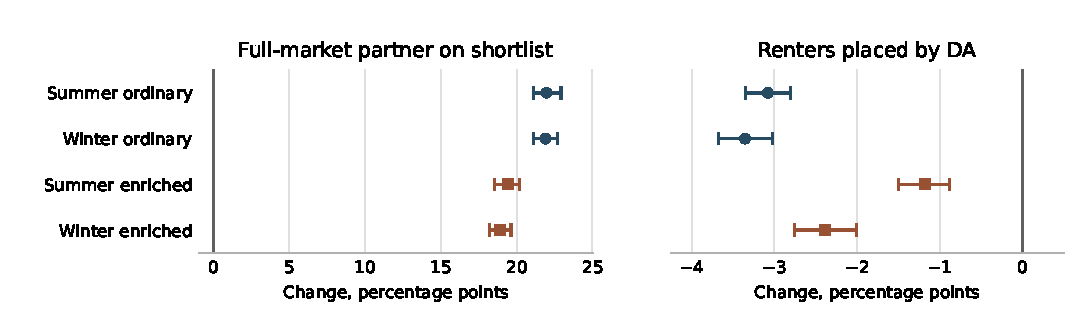
\includegraphics[width=.97\linewidth]{figures/accuracy_placement.pdf}
\caption{Replacing uniform shortlists with the contextual model for everyone. In each panel the zero line means that the two policies agree on the average rate. Whiskers are paired pointwise 95\% intervals over 48 seed blocks. Partner recovery uses renters matched under full exposure; placement uses all renters. Absolute levels and eight policies appear in Table~\ref{tab:ai}.}
\Description{In each of four panels the contextual model raises partner recovery by about twenty percentage points and reduces placement by one to four percentage points.}\label{fig:predict}\end{figure}

\paragraph{Predicting the full-market partner.}
In ordinary summer markets, the contextual rule displayed the full-market partner for 39.55\% of matched renters, against 17.58\% for uniform and 36.05\% for the pointwise model. Its advantage over pointwise was 3.51 points (paired 95\% interval $[2.98,4.04]$). Winter ordinary gave 38.27\%, 16.37\% and 34.53\% ($+3.73$ points, $[3.05,4.40]$). Context improved on pointwise by 4.40 and 4.07 points in the enriched panels. The denominator here is the set matched under full exposure. For placement rates it is every renter, including the 85.99\% and 82.70\% of lower-income renters in the two ordinary panels whose feasible set was empty.

\paragraph{Counting actual placements under the new display.}
Improving partner recovery did not increase placements relative to uniform when every renter received their five highest scores. Summer ordinary placement fell from 54.30\% to 51.22\%; winter fell from 56.18\% to 52.83\%. A coordinated anchor recovered part of that gap. In enriched markets it raised contextual placement to 69.93\% and 71.84\%, above uniform in both seasons. Even a transparent score with the same anchor reached 68.99\% and 72.07\%. An architecture-only comparison would miss how much of this improvement comes from coordinating the five slots.

\paragraph{Changing only the competitors' lists.}
In enriched markets, replacing higher-income uniform shortlists with contextual top-five shortlists raised lower-income placement from 35.89\% to 43.41\% in summer and from 39.98\% to 47.45\% in winter. In ordinary markets the corresponding changes were from 1.90\% to 1.67\% and from 2.84\% to 2.31\%. In the enriched panels a group-level gain coexists with a loss of placement for 4.95\% and 5.53\% of \emph{all} lower-income instances. Across all four panels these changes affect 2,586 previously matched instances. The scale of the net gain is sensitive to the listing-side screening assumption. Removing its income term on an eight-block paired subsample left positive enriched spillovers of 4.04 and 4.16 points, while raising lower-income placement levels in both arms (Appendix~\ref{app:income-stress}).
